\documentclass[12pt,a4paper]{article}
\setlength{\textwidth}{160mm}
\setlength{\textheight}{247mm}
\setlength{\evensidemargin}{0pt}
\setlength{\oddsidemargin}{0pt}
\setlength{\topmargin}{0pt}
\setlength{\headheight}{0pt}
\setlength{\headsep}{0pt}
\usepackage{amssymb}
\usepackage{amsmath}
\usepackage[polish]{babel}
\usepackage[T1]{fontenc}
\usepackage[utf8]{inputenc}
\usepackage{graphicx}
\usepackage{algorithm,algorithmic}
\title{Generator liczb losowych}
\author{Patryk Wojciekian}
%\date{}
\floatname{algorithm}{Algorytm}
\renewcommand{\algorithmicrequire}{\textbf{Założenia:}}
\renewcommand{\algorithmicensure}{\textbf{Wynik:}}
\begin{document}
\maketitle
\begin{abstract}
Generator liczb losowych -- program komputerowy lub układ elektroniczny generujący stacjonarny i~ergodyczny, losowy ciąg elementów binarnych zorganizowanych zwykle jako ciąg liczb losowych.
\end{abstract}
\tableofcontents
\section{Generator Fibonacciego}
\textit{Generator Fibonacciego} - jest jednym z wielu wariantów uogólnionego generatora liniowego liczb losowych \cite{klucz1}.\\
Generator korzysta z~ciągu Fibonacciego, stąd wzór:
$$
X_n=X_{n-1}+X_{n-2} \quad \verb"mod " m, \quad \verb"gdzie " n\geq 2.\\
$$
Generator Fibonacciego ma dużo lepsze parametry jakościowe od innych
generatorów liniowych, ale wymaga dużo większego nakładu obliczeń przy
generowaniu, co wiąże się z~czasem. Wadą tego generatora są duże korelacje
między wyrazami ciągu. Ciągi te spełniają warunek rozkładu, ale nie speł-
niają warunku niezależności. Wady tej można się pozbyć poprzez uogólnienie
wzoru do postaci (tzw.~lagged Fibonacci generator):
$$
X_n=X_{n-p}+X_{n-q} \quad \verb"mod " m, \quad (n\geq p, p>q,q\geq 1),
$$

\begin{figure}[h!]
\centering
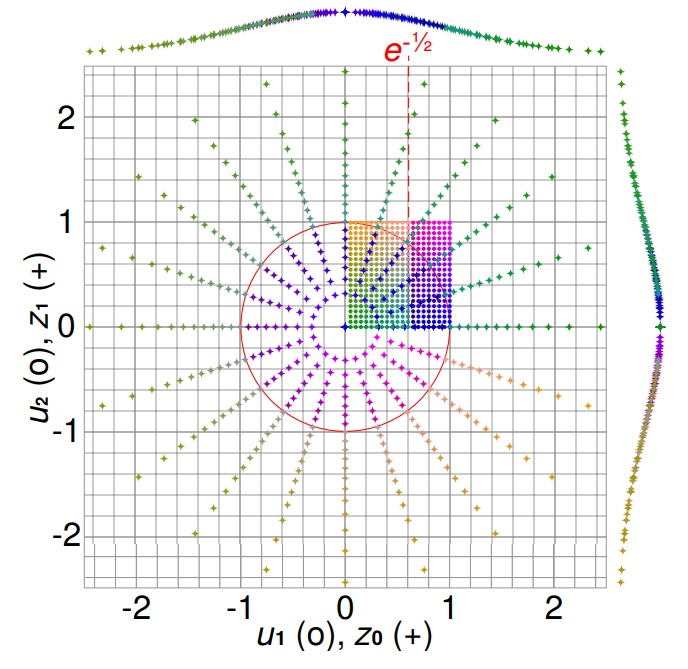
\includegraphics[scale=0.5]{obrazek}
\caption{Transformacja Boksa-Mullera}
\label{obraz1}
\end{figure}
gdzie $p$ i $q$ są opóźnieniami generatora patrz rozdział \ref{generator}.

Generator taki można jeszcze bardziej uogólnić zastępując działanie dodawania innym operatorem $\circ$ , np. operatorem odejmowania, mnożenia, XOR itd.
$$
X_n=X_{n-p}\circ X_{n-q} \quad \verb"mod " m, \quad (n\geq p, p>q,q\geq 1),
$$
generator taki oznaczamy $F(p,q,\circ )$.
\subsection{Przykład}
\label{generator}
$m = 17, p = 3, q = 1, x_0 = 7, x_1 = 16, x_2 = 5, x_n = (x_{n-p} + x_{n-q})$ mod $m$.
\begin{equation}
\begin{split}
&x_3 = (x_0 + x_2) \quad \verb"mod " 17 = (7 + 5) \quad \verb"mod " 17 = 12,\\
&x_4 = (x_1 + x_3) \quad \verb"mod " 17 = (16 + 12) \quad \verb"mod " 17 = 11,\\
&x_5 = (x_2 + x_4) \quad \verb"mod " 17 = (5 + 11) \quad \verb"mod " 17 = 16,\\
\end{split}
\end{equation}
itd.\\
Wynik obliczeń (1):  7, 16, 5, 12, 11, 16, 11, 5, 4, 15, 3, 7, \dots
\section{Transformacja Boksa-Mullera}
\textit{Transformacja Boksa-Mullera} -- metoda generowania liczb losowych o~rozkładzie normalnym, na podstawie dwóch wartości zmiennej o~rozkładzie jednostajnym w przedziale (0,1].
Niech $U_1$ oraz $U_2$ będą niezależnymi zmiennymi losowymi o rozkładzie
jednostajnym na (0, 1]. Niech zmienne $R$, $\Theta$ dane w odpowiednim układzie
współrzędnych polarnych spełniają równość $R^2 = -2 * ln U_1$ oraz $\Theta = 2\pi U_2$.
(Wówczas $R, \Theta$ są niezależne.) Połóżmy $Z_1 = R \cos\Theta = \sqrt{-2 ln U_1 \cos(2\pi U2)}$
oraz $Z_2 = R \sin\Theta = \sqrt{-2 ln U_1 \sin(2\pi U_2)}$.

Wówczas zmienne losowe $Z_1, Z_2$ są niezależne i~o~rozkładzie normalnym z
odchyleniem standardowym 1. Transformacja jest zilustrowana na rysunku \ref{obraz1}.


\section{Mersenne Twister}
Algorytm generatora liczb pseudolosowych opracowany w 1997 przez Makoto
Matsumoto i~Takuji Nishimura \cite{klucz2}. Generator jest szybki i~dostarcza wysokiej
jakości liczby pseudolosowe. Został zaprezentowany w~algorytmie \ref{algorytm}.\\
\begin{algorithm}[h!]
\caption{Algorytm ID3}
\label{algorytm}
\begin{algorithmic}[1]
\REQUIRE $index$ = 0
\ENSURE $M_T$ jest tablicą 624 elementów
\IF{$index$=0}
\FOR{i=0 \textbf{to} 623}
\STATE $y\leftarrow 32^{nd}$ bit of $M_{Ti}+$last 31 bits of $M_{T(i+1) \verb" mod " 624}$
\STATE $M_{Ti}\leftarrow M{T((i+397) \verb" mod " 624) xor (\verb" right shift by 1 bit "(y)}$
\IF{$y$ parzysta}
\STATE $M_{Ti}\leftarrow M_{Ti}$ xor $(2 567 483 615)$
\ENDIF
\ENDFOR
\ENDIF
\end{algorithmic}
\end{algorithm}

Cechy algorytmu:
\begin{itemize}
\item Zalety:
\begin{enumerate}
\item okres $2^{19937}-1$,
\item wysoki stopień równomiernego rozmieszczenia.
\end{enumerate}
\item Wady:
\begin{enumerate}
\item nie jest zbyt elegancki,
\item jest nazbyt skomplikowany w implementacji.
\end{enumerate}
\end{itemize}

\begin{table}[h!]
\centering
\begin{tabular}{rllc}
\textbf{Nr.}&\textbf{Fib}&\textbf{ID3}&\textbf{Twister} \\ \hline
1 & 31 & 84 & 66 \\
2 & 59 & 87 & 59 \\
3 & 26 & 84 & 65 \\
4 & 35 & 60 & 73 \\
5 & 13 & 29 & 41 \\ \hline 
\end{tabular}
\caption{Przykładowa tablica liczb losowych}
\label{tablica1}
\end{table}
\section{Tablica liczb losowych}
Tablica \ref{tablica1} zawiera przykładowe ciągi liczb losowych, wygenerowanych przez poszczególne algorytmy.

\begin{thebibliography}{9}
\bibitem{klucz1}  George Marsaglia, Arif Zaman, and Wai Wan Tsang: ''Toward a universal
random number generator''. Statistics \& Probability Letters. Volume 9,
Issue 1, January 1990, Pages 35-39.
\bibitem{klucz2}  Makoto Matsumoto and Takuji Nishimura, ''Mersenne twister: a 623-
dimensionally equidistributed uniform pseudorandom number generator'',
ACM Trans. Model. Comput. Simul. 8, 3 (1998).
\end{thebibliography}

\end{document}